\documentclass[xcolor=table,dvipsnames]{beamer}

\usepackage{lscape, amsmath, amsfonts, amssymb, setspace, theorem, wrapfig, graphicx, float, multirow, subfig, color, rotating, multicol, datetime, natbib, venndiagram, pstricks, xkeyval, tikz, etoolbox, verbatim, pgf, tikz, pgfplots, mathrsfs, nth}

\usepackage{listings}
\usepackage{xcolor}
\usetikzlibrary{arrows}

\definecolor{codegreen}{rgb}{0,0.6,0}
\definecolor{codegreengray}{rgb}{0,0.4,0}
\definecolor{codegray}{rgb}{0.5,0.5,0.5}
\definecolor{codeblue}{rgb}{0.00,0,0.82}
\definecolor{backcolour}{rgb}{0.95,0.95,0.92}
\definecolor{jeopardy}{rgb}{.24,.47,.914}

\lstdefinestyle{mystyle}{
    backgroundcolor=\color{backcolour},   
    commentstyle=\color{codegreengray},
    numberstyle=\tiny\color{codegray},
    stringstyle=\color{codegreen},
    basicstyle=\ttfamily\footnotesize,
    breakatwhitespace=false,         
    breaklines=true,                 
    captionpos=b,                    
    keepspaces=true,                 
    numbers=left,                    
    numbersep=5pt,                  
    showspaces=false,                
    showstringspaces=false,
    showtabs=false,                  
    tabsize=2
}
 
\lstset{style=mystyle}

\title{GV300 - Quantitative Political Analysis}
\subtitle{University of Essex - Department of Government}
\date{Week 22 -- 24 February, 2020}				% or you can specify a date, just write it down instead of "\today"
\author{Lorenzo Crippa} 

\usetheme[progressbar=frametitle]{metropolis}
\usecolortheme{seahorse}						% try others: wolverine; crane...


\begin{document}

\begin{frame}[plain]
\begin{center}
\titlepage
\end{center}
\end{frame}

\section{Question 1}

\begin{frame}
\frametitle{Question 1 -- (a)}
\begin{enumerate}
\item (a) (5 marks) What does exclusion restriction mean in the context of instrumental variable regression? \pause
\end{enumerate}

It means that the chosen instrument has an effect on the outcome variable \textbf{only} through the instrumented variable (the treatment variable)
\end{frame}

\begin{frame}
\frametitle{Question 1 -- (b)}
\begin{enumerate}
\item (b) Generate variables \texttt{X}, \texttt{T}, \texttt{Y}, \texttt{Z} and \texttt{zNot} according to the instructions. \pause Explain and demonstrate
graphically why your variable \texttt{Z} is an ideal instrumental variable. \pause Why would it be harder to demonstrate that \texttt{Z} is an ideal instrumental variable when we worked with observational data? \pause Create a variable \texttt{zNot}, which is not an ideal instrument. How would such a variable need to look like? \pause Explain and demonstrate graphically how \texttt{Z} and \texttt{zNot} differ making \texttt{zNot} a not ideal instrument.
\end{enumerate}
\end{frame}

\begin{frame}
\frametitle{Question 1 -- (b): DGP}
\begin{tikzpicture}[line cap=round,line join=round,>=triangle 45,x=1cm,y=1cm]
\clip(-1,-1) rectangle (7.5,4);
\draw [->,line width=0.6pt] (0,0) -- (2.9,0);
\draw [->,line width=0.6pt] (3,0) -- (6.9,0);
\draw [->,line width=0.6pt] (5,2) -- (3.1,0.1);
\draw [->,line width=0.6pt] (5,2) -- (6.9,0.1);
\begin{scriptsize}
\draw [fill=black] (0,0) circle (1.5pt);
\draw[color=black] (0,0.32) node {$Z$};
\draw [fill=black] (3,0) circle (1.5pt);
\draw[color=black] (3,0.33) node {$T$};
\draw [fill=black] (7,0) circle (1.5pt);
\draw[color=black] (7.2,0.10) node {$Y$};
\draw [fill=black] (5,2) circle (1.5pt);
\draw[color=black] (5,2.31) node {$X$};
\end{scriptsize}
\end{tikzpicture}  \pause

\texttt{Z} is a good instrument because it determines \texttt{T} and meets the exclusion restriction. \pause \\ With observational data it would be difficult to find a good instrument as \texttt{Z} because it is very difficult that the exclusion restriction is met. 
\end{frame}

\begin{frame}
\frametitle{Question 1 -- (b): bad instruments}
There are two ways \texttt{zNot} can be a bad instrument. \pause The first is that it has no (or weak) effect on \texttt{T}: \pause
\begin{tikzpicture}[line cap=round,line join=round,>=triangle 45,x=1cm,y=1cm]
\clip(-1,-1) rectangle (7.5,4);
\draw [dashed,->,line width=0.6pt] (0,0) -- (2.9,0);
\draw [->,line width=0.6pt] (3,0) -- (6.9,0);
\draw [->,line width=0.6pt] (5,2) -- (3.1,0.1);
\draw [->,line width=0.6pt] (5,2) -- (6.9,0.1);
\begin{scriptsize}
\draw [fill=black] (0,0) circle (1.5pt);
\draw[color=black] (0,0.32) node {$zNot$};
\draw [fill=black] (3,0) circle (1.5pt);
\draw[color=black] (3,0.33) node {$T$};
\draw [fill=black] (7,0) circle (1.5pt);
\draw[color=black] (7.2,0.10) node {$Y$};
\draw [fill=black] (5,2) circle (1.5pt);
\draw[color=black] (5,2.31) node {$X$};
\end{scriptsize}
\end{tikzpicture} 
\end{frame}

\begin{frame}
\frametitle{Question 1 -- (b): bad instruments}
The second is that the exclusion restriction is not met: \pause
\begin{tikzpicture}[line cap=round,line join=round,>=triangle 45,x=1cm,y=1cm]
\clip(-1,-1) rectangle (7.5,4);
\draw [->,line width=0.6pt] (0,0) -- (2.9,0);
\draw [->,line width=0.6pt] (0,0) -- (4.9,2);
\draw [->,line width=0.6pt] (3,0) -- (6.9,0);
\draw [->,line width=0.6pt] (5,2) -- (3.1,0.1);
\draw [->,line width=0.6pt] (5,2) -- (6.9,0.1);
\begin{scriptsize}
\draw [fill=black] (0,0) circle (1.5pt);
\draw[color=black] (0,0.32) node {$zNot$};
\draw [fill=black] (3,0) circle (1.5pt);
\draw[color=black] (3,0.33) node {$T$};
\draw [fill=black] (7,0) circle (1.5pt);
\draw[color=black] (7.2,0.10) node {$Y$};
\draw [fill=black] (5,2) circle (1.5pt);
\draw[color=black] (5,2.31) node {$X$};
\end{scriptsize}
\end{tikzpicture}  \pause

How could we solve the problem in the picture? \pause Controlling for \texttt{X}, provided we had information on that. \pause In real life, with observational data, we often \textbf{cannot} control for unobservable variable our instrument has an effect on.
\end{frame}

\begin{frame}[fragile]
\frametitle{Question 1 -- (b): coding}
R code to obtain these variables:
\begin{lstlisting}[language=R]
X <- rpois(1000, lambda = 3)
Z <- rbinom(1000, size = 8, prob = 0.4)
T <- 2 + 3*Z - 2*X + rnorm(1000)
Y <- 1 + 2*T -3*X + rnorm(1000)

model.iv <- ivreg(Y ~ T | Z)
\end{lstlisting}

Stata code:
\begin{lstlisting}[language=R]
gen X = rpoisson(3)
gen Z = rbinomial(8, 0.4)
gen T = 2 + 3*Z - 2*X + rnormal()
gen Y = 1 + 2*T -3*X + rnormal()

ivreg Y (T = Z)
\end{lstlisting}
\end{frame}

\begin{frame}[fragile]
\frametitle{Question 1 -- (b): coding}
R code to obtain bad instruments (weak):
\begin{lstlisting}[language=R]
zNot <- runif(1000)
T <- 2 + 3*Z - 2*X + 0*zNot + rnorm(1000) 
# zNot is not a cause of T
Y <- 1 + 2*T -3*X + rnorm(1000)

model.iv.bad <- ivreg(Y ~ T | zNot)
\end{lstlisting}

Stata code:
\begin{lstlisting}
gen zNot = runiform()
gen T = 2 + 3*Z - 2*X + 0*zNot + rnormal()
gen Y = 1 + 2*T -3*X + rnormal()

ivreg Y (T = zNot)
\end{lstlisting}
\end{frame}

\begin{frame}[fragile]
\frametitle{Question 1 -- (b): coding}
R code to obtain bad instruments (exclusion restriction violated):
\begin{lstlisting}[language=R]
X <- 1 + 2*zNot + rnorm(1000)
T <- 2 + 3*Z - 2*X + 5*zNot + rnorm(1000) 
# zNot IS a cause of T but also of X 
Y <- 1 + 2*T -3*X + rnorm(1000)

model.iv.bad2 <- ivreg(Y ~ T | zNot)
\end{lstlisting}

Stata code:
\begin{lstlisting}
gen X = 1 + 2*zNot + rnormal()
gen T = 2 + 3*Z - 2*X + 5*zNot + rnormal()
gen Y = 1 + 2*T -3*X + rnormal()

ivreg Y (T = zNot)
\end{lstlisting}
\end{frame}

\begin{frame}
\frametitle{Results}
\begin{table}
\begin{center}
\begin{tabular}{l c c c c }
\hline
 & Linear  & Good IV & Weak IV & Exclusion \\
 & (controls)		&		   &		 & Restriction \\
\hline
(Intercept) & $0.98^{***}$  & $-8.19^{***}$ & $-37.53$   & $36.62^{**}$ \\
            & $(0.11)$      & $(0.26)$      & $(250.76)$ & $(16.59)$    \\
T           & $1.99^{***}$  & $2.05^{***}$  & $7.27$     & $-2.14$      \\
            & $(0.01)$      & $(0.04)$      & $(44.61)$  & $(1.65)$     \\
X           & $-2.99^{***}$ &               &            &              \\
            & $(0.02)$      &               &            &              \\
\hline
R$^2$       & 1.00          & 0.89          & -2.04      & -2.55        \\
Adj. R$^2$  & 1.00          & 0.89          & -2.04      & -2.55        \\
Num. obs.   & 1000          & 1000          & 1000       & 1000         \\
\hline
\multicolumn{5}{l}{\scriptsize{$^{***}p<0.01$, $^{**}p<0.05$, $^*p<0.1$}}
\end{tabular}
\end{center}
\end{table}
\end{frame}

\section{Question 2}

\frame{
\frametitle{Question 2}
Create a dataset with 50,000 observations. Create a variable called $Instrument$, which takes a value of 0 60\% of the time and a value of 1 otherwise. \pause Generate a variable $ObservableThing \sim N(0; 1)$ and a variable $UnobservableThing$ which is also $\sim N(0; 1)$. \pause Create the variable $VariableOfInterest$, which equals 1 if $ObservableThing + UnobservableThing + Instrument \geq 2.5$ and which equals 0 otherwise. \pause Finally, generate $OutcomeVariable = UnobservableThing + VariableofInterest + e$, where $e \sim N(0; 1)$.
}

\begin{frame}{Question 2 -- Data Generating Process (causal diagram)}
\begin{tikzpicture}[line cap=round,line join=round,>=triangle 45,x=1cm,y=1cm]
\clip(-1,-4) rectangle (9,4);
\draw [->,line width=0.6pt] (0,0) -- (2.9,0);
\draw [->,line width=0.6pt] (3,0) -- (6.9,0);
\draw [->,line width=0.6pt] (1.5,2) -- (3,0.1);
\draw [->,line width=0.6pt] (5,-2) -- (3.1,-0.1);
\draw [->,line width=0.6pt] (5,-2) -- (6.9,-0.1);
\begin{scriptsize}
\draw [fill=black] (0,0) circle (1.5pt);
\draw[color=black] (0.22,0.32) node {$Instrument$};
\draw [fill=black] (3,0) circle (1.5pt);
\draw[color=black] (4.2,0.33) node {$VariableOfInterest$};
\draw [fill=black] (7,0) circle (1.5pt);
\draw[color=black] (7.4,0.33) node {$OutcomeVariable$};
\draw [fill=black] (1.5,2) circle (1.5pt);
\draw[color=black] (1.66,2.31) node {$ObservableThing$};
\draw [fill=black] (5,-2) circle (1.5pt);
\draw[color=black] (5,-2.3) node {$UnobservableThing$};
\end{scriptsize}
\end{tikzpicture}
\end{frame}

\begin{frame}[fragile]
\frametitle{Question 2 -- Data Generating Process (code)}
In R:
\begin{lstlisting}[language=R]
Instrument <- rbinom(50000, size = 1, prob = 0.4)
ObservableThing <- rnorm(50000)
UnobservableThing <- rnorm(50000)

VariableOfInterest <-ifelse(ObservableThing + UnobservableThing + Instrument >= 2.5, 1, 0)

OutcomeVariable = UnobservableThing + 1 * VariableOfInterest + rnorm(50000)
\end{lstlisting}
\end{frame}

\begin{frame}[fragile]
\frametitle{Question 2 -- Data Generating Process (code)}
In Stata:
\begin{lstlisting}
gen Instrument = rbinomial(1, 0.4)
gen ObservableThing = rnormal()
gen UnobservableThing = rnormal()

gen VariableOfInterest = (ObservableThing + UnobservableThing + Instrument >= 2.5)

gen OutcomeVariable = UnobservableThing + 1 * VariableOfInterest + rnormal()
\end{lstlisting}
\end{frame}

\begin{frame}
\frametitle{Question 2 (a)}
\begin{enumerate}
\item[2.](a) (5 Marks) What is the causal effect of $VariableOfInterest$ on $OutcomeVariable$?
\end{enumerate} \pause

Remember the equation that defines $OutcomeVariable$: $OutcomeVariable = UnobservableThing + VariableofInterest + e$ \pause 

The causal effect will have a size of $1$!
\end{frame}

\begin{frame}
\frametitle{Question 2 (b)}
\begin{enumerate}
\item[2.] (b) (5 Marks) Regress $OutcomeVariable$ on $VariableOfInterest$ and interpret the coefficient. Why is this not close to the causal effect from part (a)?
\end{enumerate} \pause

Model: \pause $OutcomeVariable = \alpha + \beta VariableOfInterest + u$ \pause

The coefficient does not provide the causal effect of 1 from part (a) because we have $UnobservableThing$ which is a confounder and: \pause 
\begin{enumerate}
\item we are neither controlling for it \pause
\item nor instrumenting $VariableOfInterest$
\end{enumerate} \pause
(I'll show all results together at the end of Question 2)
\end{frame}

\begin{frame}
\frametitle{Question 2 (c)}
\begin{enumerate}
\item[2.] (c) (10 Marks) Use $Instrument$ as the instrumental variable for $VariableOfInterest$ in the regression of $OutcomeVariable$ on $VariableOfInterest$. Calculate the causal effect of $VariableOfInterest$ on $OutcomeVariable$ both by hand and using the proper commands in Stata or R. Comment on what you observe.
\end{enumerate} \pause

2SLS model: \pause \\
$\widehat{VariableOfInterest} = \hat{\gamma} + \hat{\delta} Instrument$ \pause
$OutcomeVariable = \hat{\alpha} + \hat{\beta} \widehat{VariableOfInterest} + \hat{u}$ \pause

Also remember that the instrumented unbiased effect of $T_i$ is: \pause
$$d=\frac{Cov(Y_i,Z_i)}{Cov(T_i,Z_i)} $$
\end{frame}

\begin{frame}[fragile]
\frametitle{Question 2 (c)}
Code in R:
\begin{lstlisting}[language=R]
# 1st and 2nd stage
first.st <- lm(VariableOfInterest ~ Instrument)
fitted.var <- first.st$fitted.values
second.st <- lm(OutcomeVariable ~ fitted.var)

model.iv <- ivreg(OutcomeVariable ~ VariableOfInterest | Instrument)
\end{lstlisting} \pause

Code in Stata:
\begin{lstlisting}
reg VariableOfInterest Instrument
predict fitted_var
reg OutcomeVariable fitted_var

ivreg OutcomeVariable (VariableOfInterest=Instrument)
\end{lstlisting}
\end{frame}

\begin{frame}[fragile]
\frametitle{Question 2 (c) -- Comparison of results}
\begin{table}
\begin{center}
\begin{tabular}{l c c }
\hline
 & Manually & \texttt{ivreg} \\
\hline
(Intercept)        & $0.02$       & $0.02$       \\
                   & $(0.01)$     & $(0.01)$     \\
VariableOfInterest & $0.91^{***}$ & $0.91^{***}$ \\
                   & $(0.13)$     & $(0.13)$     \\
\hline
Adj. R$^2$         & 0.00         & 0.11         \\
Num. obs.          & 50000        & 50000        \\
\hline
\multicolumn{3}{l}{\scriptsize{$^{***}p<0.01$, $^{**}p<0.05$, $^*p<0.1$}}
\end{tabular}
\end{center}
\end{table} \pause
Two notes: \pause
\begin{enumerate}
\item SEs will be slightly different because of the different vCov matrices, but parameters will be \emph{identical} \pause
\item $R^{2}$ in the \nth{1} model. We have a good instrument yet the variation we explain is low. \pause Don't over-trust the $R^{2}$!
\end{enumerate}
\end{frame}

\begin{frame}[fragile]
\frametitle{Question 2 (d)}
\begin{enumerate}
\item[2.] (d) (10 Marks) Change the setup from part (a) such that $Instrument$ is only equal to 1 2\% of the time. Then rerun the regression in part (c) (using Stata or R) and comment on what happens. What's wrong with this instrument?
\end{enumerate} \pause

If we only change the instrument and do not change the rest of the DGP, we will have a new instrument which will be very weakly correlated with the previous one and thus with $OutcomeVariable$, thus it will give us a bad estimate of the causal effect of $VariableOfInterest$
\end{frame}

\begin{frame}[fragile]
\frametitle{Question 2 (d)}
Code in R:
\begin{lstlisting}[language=R]
Instrument2 <- rbinom(50000, size = 1, prob = 0.02)
cor(Instrument, Instrument2) # 0.0015: very very low!
cor(VariableOfInterest, Instrument2) # 0.0053: very low too

model.iv.weak <- ivreg(OutcomeVariable ~ VariableOfInterest | Instrument2)
\end{lstlisting} \pause

Code in Stata:
\begin{lstlisting}
gen Instrument2 = rbinomial(1, 0.02)
corr Instrument Instrument2
corr VariableOfInterest Instrument2

ivreg OutcomeVariable (VariableOfInterest = Instrument2)
\end{lstlisting}
\end{frame}

\begin{frame}
\frametitle{Question 2 (e)}
\begin{enumerate}
\item[2.](e) (10 Marks) Change the setup from part a such that $VariableOfInterest = Obs.Thing + Unobs.Thing + 0.05*Instr.$ where $Instrument$ still takes a value of 0 60\% of the time and a value of 1 otherwise. Then rerun the regression in part (c) (using Stata or R) and comment on what happens.
\end{enumerate}\pause

The instrument will be a very weak determinant of $VariableOfInterest$ (its causal effect is of size $0.05$). \pause Thus it will give us a biased estimate of the causal effect of $VariableOfInterest$ on $OutcomeVariable$
\end{frame}

\begin{frame}[fragile]
\frametitle{Question 2 (e)}
Code in R:
\begin{lstlisting}[language=R]
VariableOfInterest = ObservableThing + UnobservableThing + 0.05*Instrument
model.iv2 <- ivreg(OutcomeVariable ~ VariableOfInterest | Instrument)
\end{lstlisting} \pause

Code in Stata:
\begin{lstlisting}
gen VariableOfInterest = ObservableThing + UnobservableThing + 0.05*Instrument
ivreg OutcomeVariable (VariableOfInterest = Instrument)
\end{lstlisting}
\end{frame}

\begin{frame}
\frametitle{Question 2 (f)}
\begin{enumerate}
\item[2.](f) (10 Marks) Change the setup from part a such that $OutcomeVariable = Unobs.Thing + Var.ofInt. + 0.05*Instr. + e$ where $Instrument$ still takes a value of 0 60\% of the time and a value of 1 otherwise. Then rerun the regression in part (c) (using Stata or R) and comment on what happens.
\end{enumerate}\pause

The instrument will be a determinant of $OutcomeVariable$, exclusion restriction is not met. \pause

Even if its causal effect on $OutcomeVariable$ will be weak ($0.05$), this will be enough to bias the estimate of the causal effect of $VariableOfInterest$ when it is instrumented using $Instrument$.
\end{frame}

\begin{frame}[fragile]
\frametitle{Question 2 (e)}
Code in R:
\begin{lstlisting}[language=R]
OutcomeVariable = UnobservableThing + VariableOfInterest + 0.05*Instrument + rnorm(50000)
model.iv3 <- ivreg(OutcomeVariable ~ VariableOfInterest | Instrument)
\end{lstlisting} \pause

Code in Stata:
\begin{lstlisting}
gen OutcomeVariable = UnobservableThing + VariableOfInterest + 0.05*Instrument + rnormal()

ivreg OutcomeVariable (VariableOfInterest = Instrument)
\end{lstlisting}
\end{frame}

\begin{frame}
\frametitle{Question 2 -- comparison of results}
\begin{table}
\begin{center}
\begin{tabular}{l c c c c c }
\hline
 & (b) 			& (c) 		& (d) & (e) & (f) \\
\hline
(Intercept)        & $-0.10^{***}$ & $0.02$       & $-0.53$  & $-0.01$      & $-0.02$      \\
                   & $(0.01)$      & $(0.01)$     & $(0.49)$ & $(0.04)$     & $(0.02)$     \\
VariableOfInterest & $2.34^{***}$  & $0.91^{***}$ & $7.70$   & $3.15^{***}$ & $2.47^{***}$ \\
                   & $(0.02)$      & $(0.13)$     & $(6.20)$ & $(1.18)$     & $(0.57)$     \\
\hline
R$^2$              & 0.18          & 0.11         & -0.75    & -5.40        & 0.43         \\
Adj. R$^2$         & 0.18          & 0.11         & -0.75    & -5.40        & 0.43         \\
Num. obs.          & 50000         & 50000        & 50000    & 50000        & 50000        \\
\hline
\multicolumn{6}{l}{\scriptsize{$^{***}p<0.01$, $^{**}p<0.05$, $^*p<0.1$}}
\end{tabular}
\end{center}
\end{table}
\end{frame}

\section{Question 3}

\begin{frame}
\frametitle{Question 3}
\texttt{USStateLegislature.csv}: 
\begin{itemize}
\item vote share of the female candidates in U.S. state legislature elections (\texttt{votemargin}) by electoral district \pause 
\item turnout \textbf{among women in the NEXT election} by electoral district. (\texttt{turnout}). \pause
\item vote share of the democratic presidential candidate in that electoral district and year (\texttt{democraticvoteshare$\_$president}). \pause
\end{itemize}

Res. Q: \textcolor{red}{Is there an effect of having women enter elected office in one election cycle on women's turnout in the next election cycle?} 
\end{frame}

\begin{frame}
\frametitle{Question 3 (a)}
\begin{enumerate}
\item[3.] (a) (3 marks) Generate a scatter plot \texttt{turnout} vs \texttt{votemargin} and add a vertical line at $votemargin=0$. What do you see? \pause
\end{enumerate}

\begin{center}
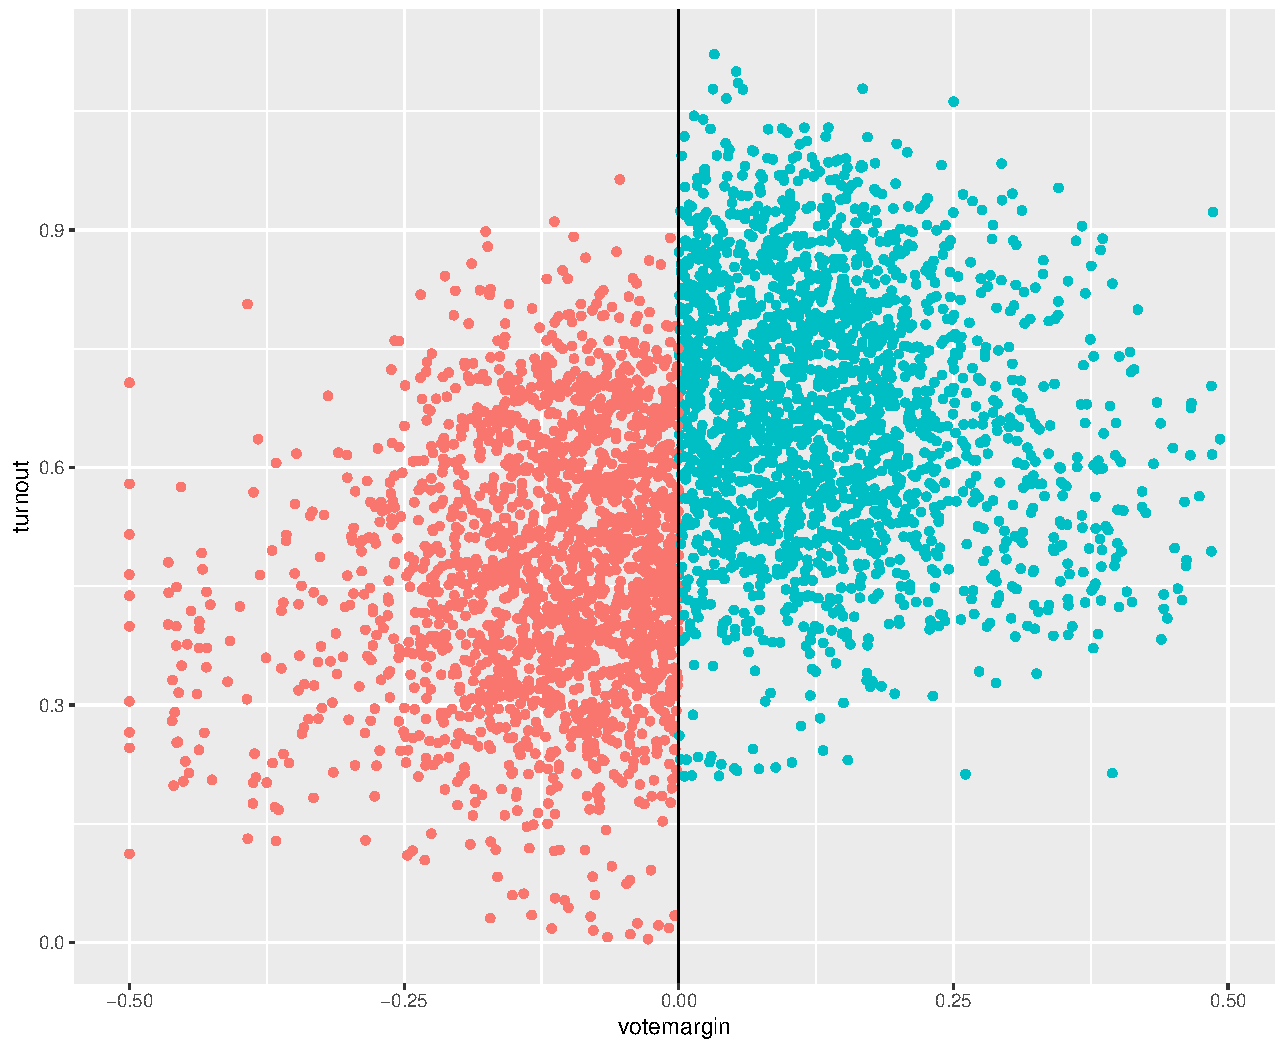
\includegraphics[width=80mm]{pictures/week_22_3scatt.pdf} 
\end{center}
\end{frame}

\begin{frame}[fragile]
\frametitle{Question 3 (a) -- coding}
In R (I use the \texttt{indicator} variable from point b):
\begin{lstlisting}[language=R]
data %>% ggplot(aes(y = turnout, x = votemargin)) + geom_point(aes(colour = indicator)) + 
  geom_vline(xintercept = 0) + theme(legend.position = "none") # this way we get rid of the legend
\end{lstlisting} \pause

In Stata:
\begin{lstlisting}
twoway ///
	(scatter turnout votemargin if votemargin >= 0) ///
	(scatter turnout votemargin if votemargin < 0), xline(0) leg(off)
\end{lstlisting} \pause

Districts where female candidates barely lost have a generally lower female turnout in the subsequent election than those were female candidates barely won
\end{frame}

\begin{frame}
\frametitle{Question 3 (b)}
\begin{enumerate}
\item[3.] (b) (7 marks) Draw lines through the data cloud below and above $votemargin=0$. Lay a locally smoothed curve, a linear fit line, or a quadratic fit line over the scatter plot. What line approximates the data best (just eyeball)?
\end{enumerate}
\end{frame}

\begin{frame}[fragile]
\frametitle{Question 3 (b) -- coding in R}
Various types of fit lines:
\begin{lstlisting}[language=R]
# indicator:
data$indicator[data$votemargin >= 0] <- 1
data$indicator[data$votemargin < 0] <- 0

# first save plot:
p <- data %>% ggplot(aes(y = turnout, x = votemargin)) + geom_point(aes(colour = indicator)) + 
  geom_vline(xintercept = 0) + theme(legend.position = "none")

# different fits:
p + geom_smooth(aes(group = indicator))
p + geom_smooth(aes(group = indicator), method = "lm")
p + geom_smooth(aes(group = indicator), method = "lm", formula = y ~ x + I(x^2))
\end{lstlisting}
\end{frame}

\begin{frame}[fragile]
\frametitle{Question 3 (b) -- coding in Stata}
Various types of fit lines:
\begin{lstlisting}
* linear model
twoway (scatter turnout votemargin if votemargin >= 0) ///
	(scatter turnout votemargin if votemargin < 0) ///
	(lfit turnout votemargin if votemargin >= 0) ///
	(lfit turnout votemargin if votemargin < 0), xline(0) leg(off)

* quadratic model
twoway (scatter turnout votemargin if votemargin >= 0) ///
	(scatter turnout votemargin if votemargin < 0) ///
	(qfit turnout votemargin if votemargin >= 0) ///
	(qfit turnout votemargin if votemargin < 0), xline(0) leg(off)
\end{lstlisting}
\end{frame}

\begin{frame}
\frametitle{Question 3 (b) -- Locally smoothed fit}
\centering
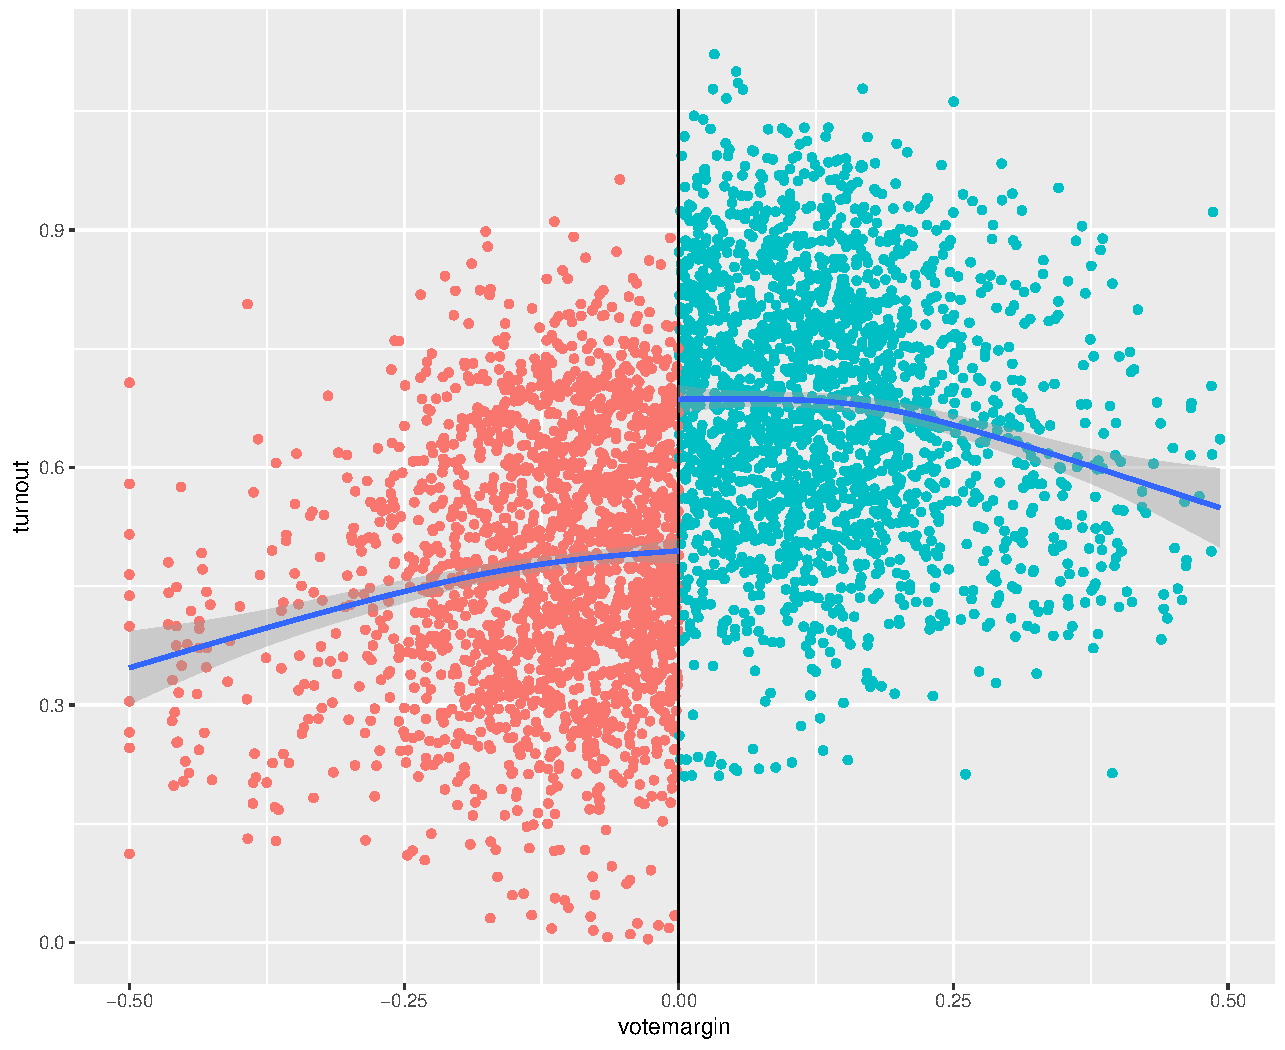
\includegraphics[width=100mm]{pictures/week_22_3locfit.pdf} 
\end{frame}

\begin{frame}
\frametitle{Question 3 (b) -- Linear fit}
\centering
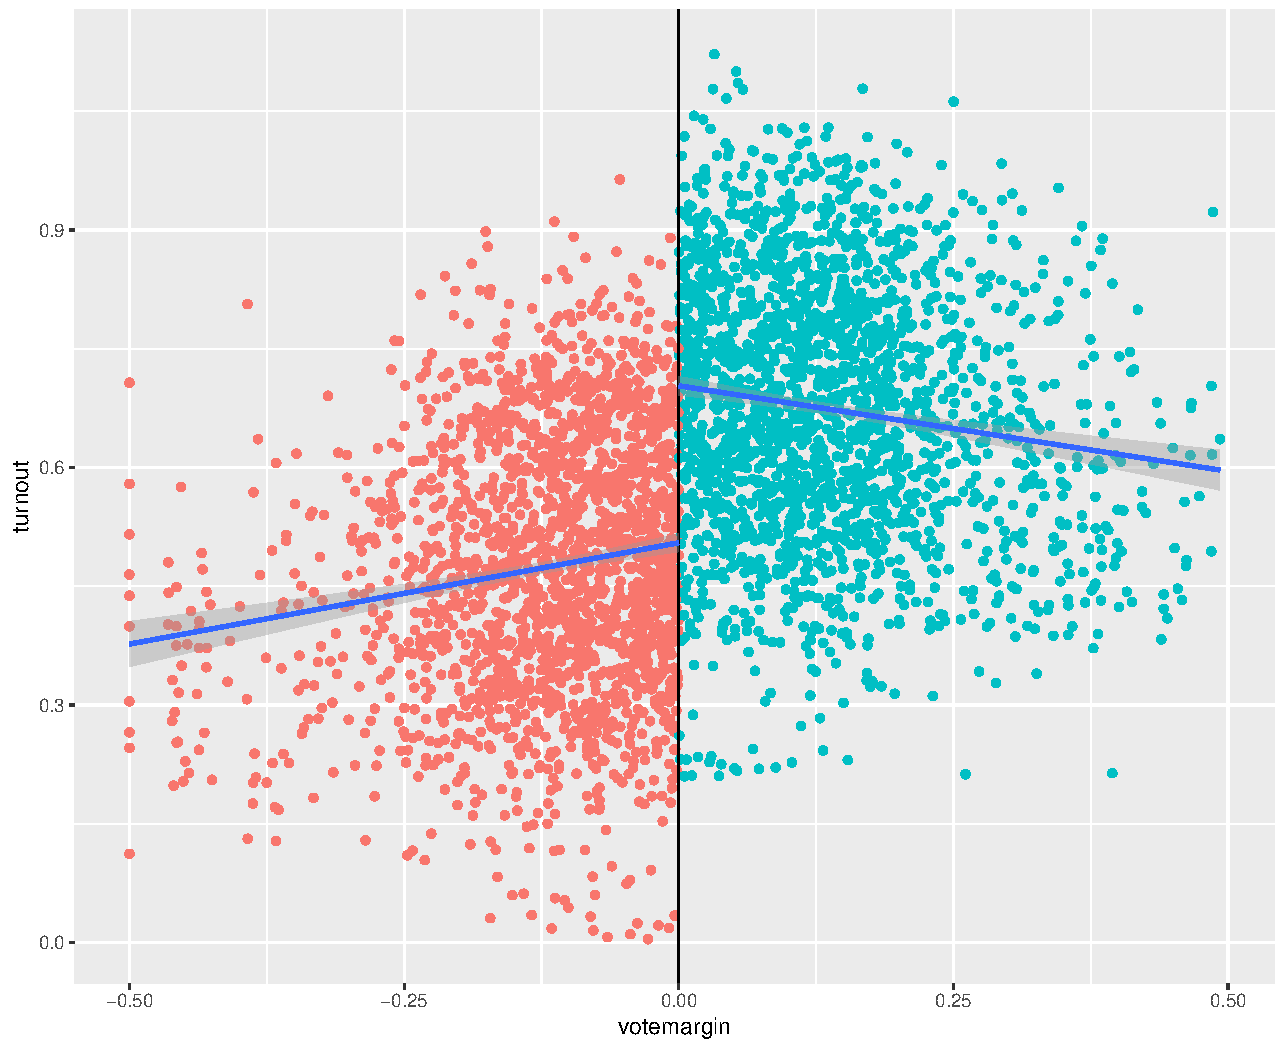
\includegraphics[width=100mm]{pictures/week_22_3linfit.pdf} 
\end{frame}

\begin{frame}
\frametitle{Question 3 (b) -- Quadratic fit}
\centering
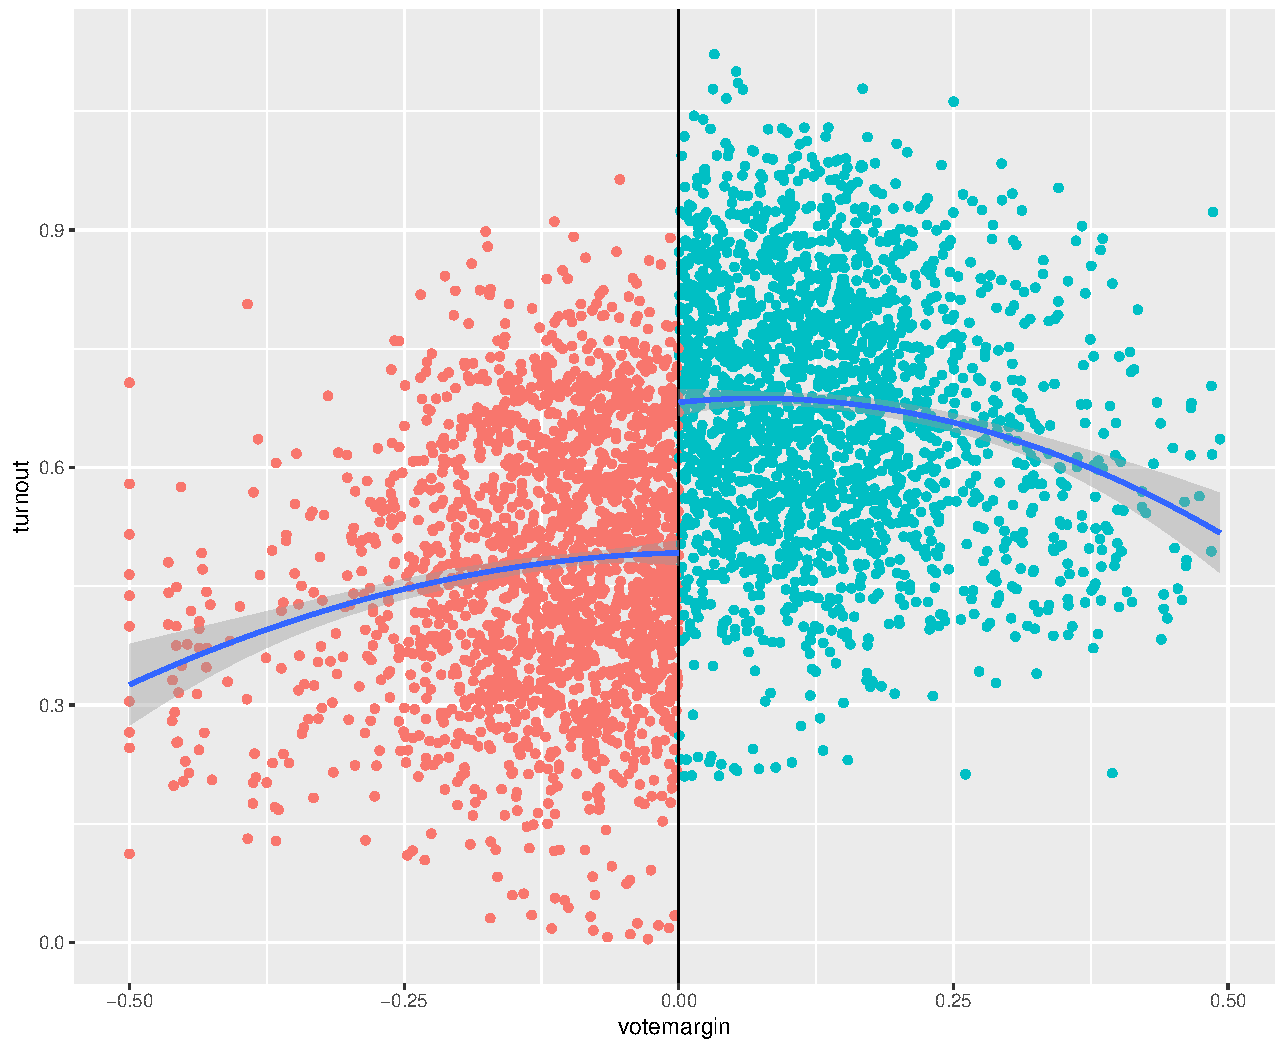
\includegraphics[width=100mm]{pictures/week_22_3sqrfit.pdf} 
\end{frame}

\begin{frame}
\frametitle{Question 3 (c)}
\begin{enumerate}
\item[3.] (c) (15 marks) Estimate the effect of having a woman enter elected office on female turnout. \pause
	\begin{itemize}
	\item For R, use the \texttt{RDestimate} command from the \texttt{rdd} package. \pause
	\item In Stata use \texttt{rdrobust} command (type \texttt{findit rdrobust}) \pause 
	\end{itemize}
Set a proper cut-point for the forcing variable \texttt{votemargin}. \pause
	\begin{itemize}
	\item What is the estimated causal effect of a woman elected to the legislature on \texttt{turnout}? \pause
	\item What type of average treatment effect are you estimating here? \pause
	\end{itemize} 
In R and Stata you can specify different bandwidth manually or choose between different bandwidth selection mechanism for estimation. \pause
	\begin{itemize}
	\item What does bandwidth selection have to do with the trade-off between variance and bias of the estimate of the causal effect? 
	\end{itemize}
\end{enumerate}
\end{frame}

\begin{frame}[fragile]
\frametitle{Question 3 (c) -- coding}
In R:
\begin{lstlisting}[language=R]
model <- RDestimate(turnout ~ votemargin, data = data, cutpoint = 0, se.type = "HC1")

# specify bandwidth:
model2 <- RDestimate(turnout ~ votemargin, data = data, cutpoint = 0, bw = c(0.10), se.type = "HC1")
\end{lstlisting}\pause

In Stata:
\begin{lstlisting}
rdrobust turnout votemargin, c(0)  vce(hc1)

* specify bandwidth:
rdrobust turnout votemargin, c(0) b(-.2 .2)  vce(hc1)
\end{lstlisting}
\end{frame}

\begin{frame}[fragile]
\frametitle{Question 3 (c) -- results}
\begin{small}
\begin{verbatim}
           Bd.w.   Obs.  Estimates   SE.         
LATE       0.2038  3296  0.1926 ***  0.011916 
Half-BW    0.1019  1830  0.2008 ***  0.016068 
Double-BW  0.4076  3999  0.1951 ***  0.009649 
---
Signif. codes:  0 '***' 0.001 '**' 0.01 '*' 0.05 '.' 0.1

F-statistics:
           F      Num. DoF  Denom. DoF  p
LATE       393.7  3         3292        0
Half-BW    212.8  3         1826        0
Double-BW  502.4  3         3995        0
\end{verbatim}
\end{small}\pause

Here we are estimating a \textbf{Local} Average Treatment Effect \pause \\
Trade-off: enlarging the bandwith gives us more observations (smaller variance), but the unobservable confounders get stronger
\end{frame}

\begin{frame}
\frametitle{Question 3 (d)}
\begin{enumerate}
\item[3.] (d) (15 marks) For assessing the validity of the RDD estimate of the causal effect it is crucial to check whether the assumptions allowing RDD to make causal claims are met. 
The three most important assumptions are \pause
\begin{enumerate}
\item[(1)] The assignment of $T_i$ by the forcing variable $x_i$ is not manipulable. 
\item[(2)] Treatment effect only occurs at cut-off $x_0$ not at other cut-offs. 
\item[(3)] $T_i$ only affects the outcome variable $Y_i$ but not any other non-outcome covariates. \pause
\end{enumerate}
Here are your tasks: 
\begin{enumerate}
\item[i.] Explain the meaning of each assumption in your own words in 2-3 sentences. 
\item[ii.] Which of these three assumptions can be empirical tested?
\item[iii.] Provide empirical tests for those assumptions you identified in (ii.) that can be tested using \texttt{USStateLegislature.csv}.
\end{enumerate}
\end{enumerate}
\end{frame}

\begin{frame}
\frametitle{Question 3 (d) -- i and ii}
\begin{enumerate}
\item[(1)] The assignment of $T_i$ by the forcing variable $x_i$ is not manipulable. \pause No observation $i$ can self-select in either being ``treated'' or not (begin below or above the threshold). \pause Otherwise unobservable factors accounting for the self-selection should be modelled! \pause \textbf{We cannot test it} \pause
\item[(2)] Treatment effect only occurs at cut-off $x_0$ not at other cut-offs. \pause There are no other cut-off points that could be used to distinguish between treatment and control groups, and the cut-off is the same for all observations. \pause \textbf{We can test it} \pause
\item[(3)] $T_i$ only affects the outcome variable $Y_i$ but not any other non-outcome covariates. \pause The effect isolated by the threshold is uniquely determined by the treatment variable and impacts only the outcome variable. \pause All other covariates remain unchanged. \pause \textbf{We can test it so far as we have information on the covariates}
\end{enumerate}
\end{frame}

\begin{frame}[fragile]
\frametitle{Question 3 (d) -- iii -- Test assumption 2} \pause
We can run different models testing different cut-off points and expect to have \textbf{no} significant result \pause

In R:
\begin{lstlisting}[language=R]
RDestimate(turnout~votemargin,cutpoint=-.1,data=data, se.type = "HC1") # not significant
RDestimate(turnout~votemargin,cutpoint=.1,data=data, se.type = "HC1") # not significant
\end{lstlisting} \pause

In Stata:
\begin{lstlisting}[language=R]
rdrobust turnout votemargin, c(-.1) vce(hc1)
rdrobust turnout votemargin, c(.1) vce(hc1)
\end{lstlisting}
\end{frame}

\begin{frame}[fragile]
\frametitle{Question 3 (d) -- iii -- Test assumption 3} \pause
Re-run all the analysis using covariates as dependent variables (hopefully no significant results). \pause

In R: 
\begin{lstlisting}[language=R]
data %>% ggplot(aes(y=democraticvoteshare_president,x=votemargin)) + geom_point(aes(col = indicator)) +
  geom_vline(xintercept=0)
RDestimate(democraticvoteshare_president ~ votemargin, cutpoint = 0, data = data, se.type = "HC1")
\end{lstlisting} \pause

In Stata:
\begin{lstlisting}[language=R]
twoway (scatter democraticvoteshare_president votemargin if votemargin >= 0) ///
	(scatter democraticvoteshare_president votemargin if votemargin < 0), xline(0) leg(off)
rdrobust democraticvoteshare_president votemargin, c(0)  vce(hc1)
\end{lstlisting}
\end{frame}

\begin{frame}
\frametitle{Question 3 (d) -- iii -- Test assumption 3}
\centering
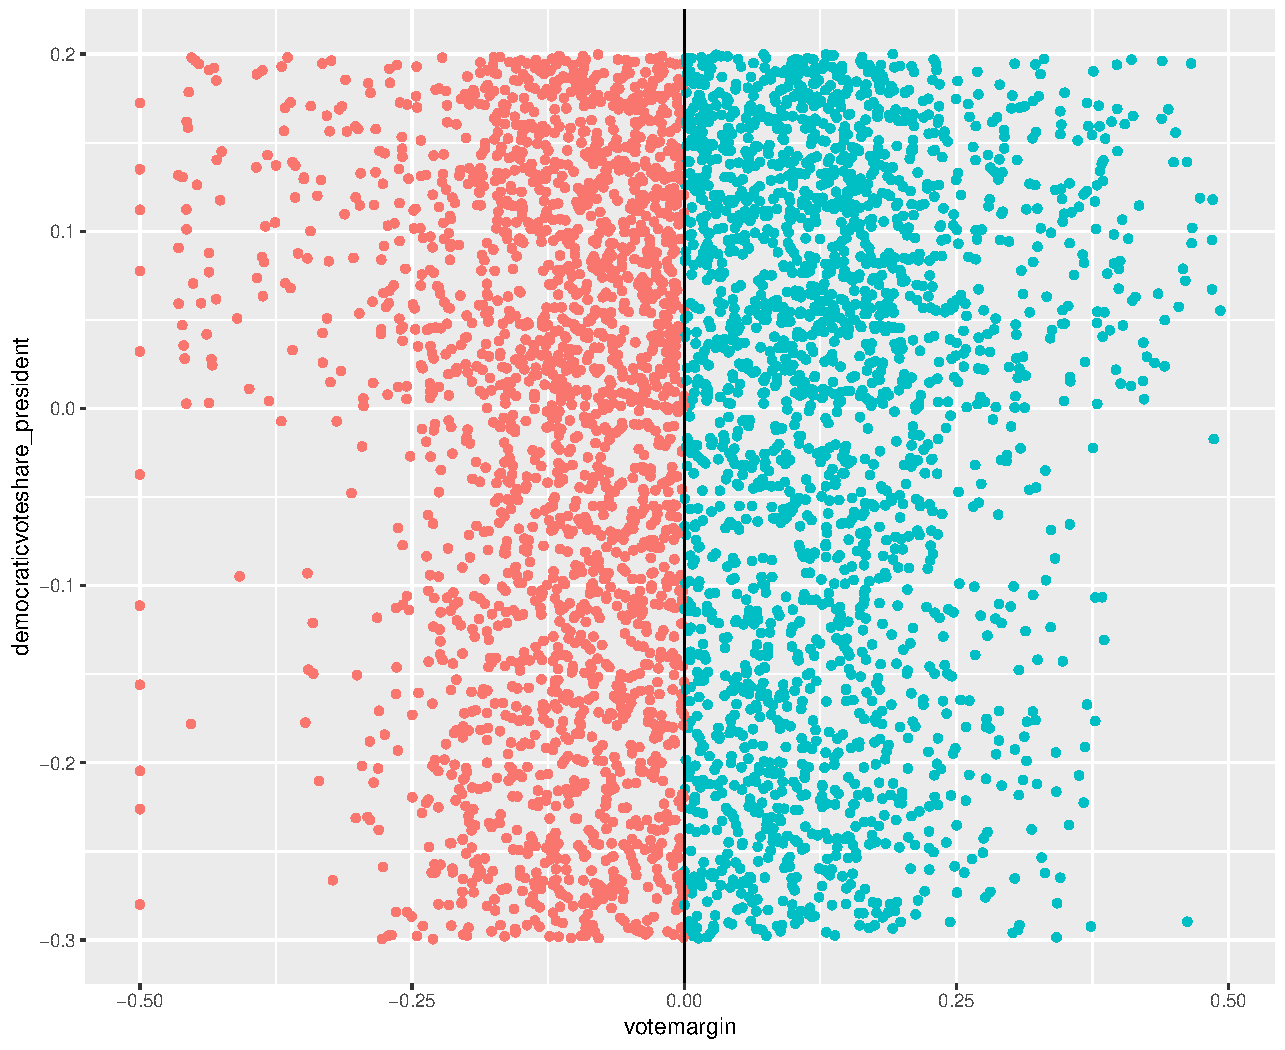
\includegraphics[width=100mm]{pictures/week_22_ass3.pdf} 
\end{frame}

\begin{frame}[fragile]
\frametitle{Question 3 (d) -- iii -- Test assumption 1?} 
Assumption 1: \pause
\begin{itemize}
\item In principle not testable \pause 
\item Yet, we can get some \textbf{evidence} that could speak to it \pause 
\item The assumption tells us that manipulation/sorting into T and C is not possible: evaluate by density plot. \pause
\item If there is no increased density around the cut-off, we probably do not observe manipulation.
\end{itemize} \pause

In R: \pause
\begin{lstlisting}[language=R]
DCdensity(data$votemargin,0, verbose=T, plot=T)
\end{lstlisting} \pause

The command comes with a test of the null-hypothesis that there is no
difference in the densities before and after the discontinuity. We do not reject the null ($p-value = 0.17$) \pause Unfortunately I could not find any equivalent command in Stata
\end{frame}

\begin{frame}
\frametitle{Question 3 (d) -- iii -- Test assumption 1?}
\centering
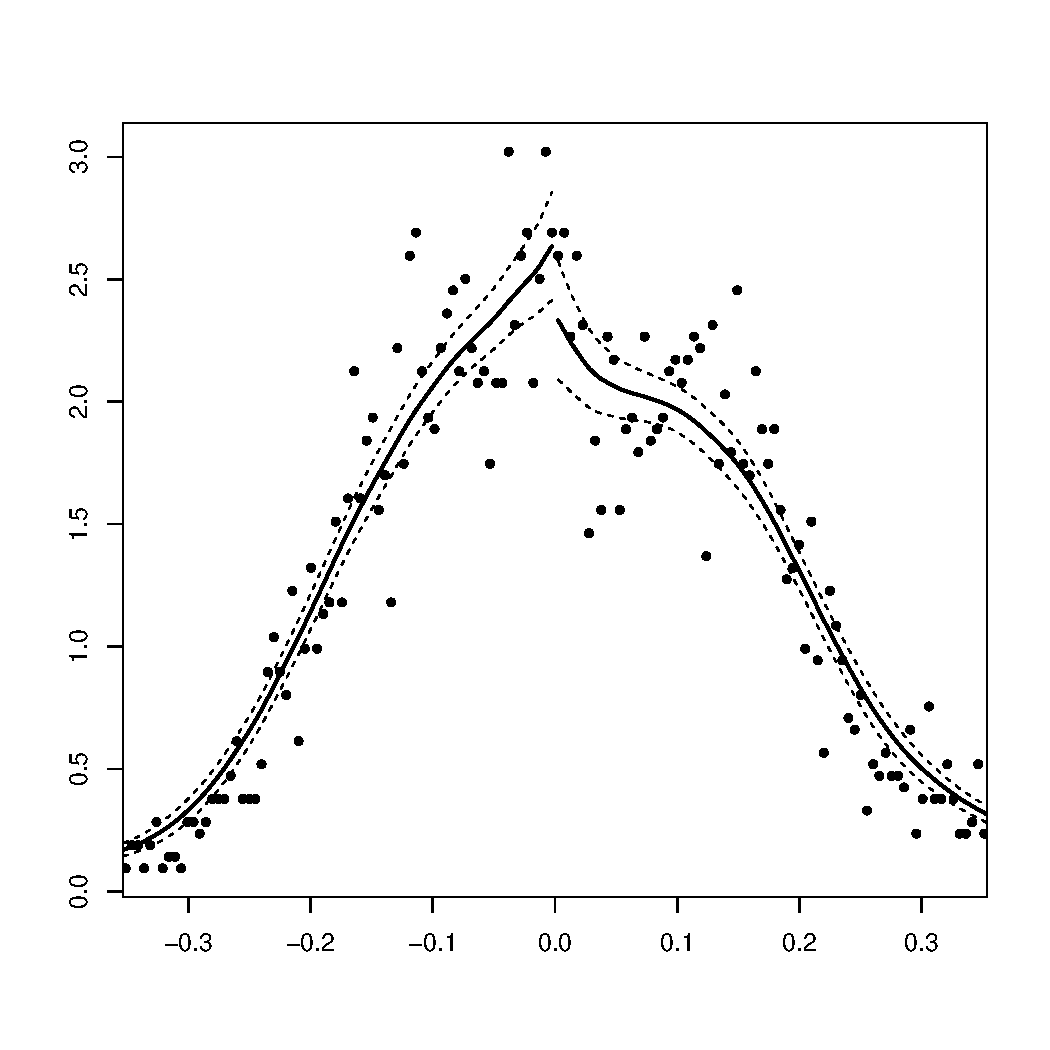
\includegraphics[width=80mm]{pictures/week_22_ass1.pdf} 
\end{frame}

\section{Question 4}

\begin{frame}
\frametitle{Question 4}
\centering
\textbf{Your research project}: \pause Always feel free to ask me specific questions if you have them, or pass by my office during academic support hour.
\end{frame}

\frame{
\frametitle{Conclusion}
\begin{center}
All clear? More questions? \\
Thanks and see you next week!
\end{center}
}

\end{document}